\def\year{2020}\relax
%File: formatting-instruction.tex
\documentclass[letterpaper]{article} % DO NOT CHANGE THIS
\usepackage{aaai20}  % DO NOT CHANGE THIS
\usepackage{times}  % DO NOT CHANGE THIS
\usepackage{helvet} % DO NOT CHANGE THIS
\usepackage{courier}  % DO NOT CHANGE THIS
\usepackage[hyphens]{url}  % DO NOT CHANGE THIS
\usepackage{graphicx} % DO NOT CHANGE THIS
\usepackage{algorithm,algorithmic}
\usepackage{amsmath,amssymb,amsfonts}
\usepackage{subcaption}
\captionsetup{compatibility=false}
\urlstyle{rm} % DO NOT CHANGE THIS
\def\UrlFont{\rm}  % DO NOT CHANGE THIS
\usepackage{graphicx}  % DO NOT CHANGE THIS
\frenchspacing  % DO NOT CHANGE THIS
\setlength{\pdfpagewidth}{8.5in}  % DO NOT CHANGE THIS
\setlength{\pdfpageheight}{11in}  % DO NOT CHANGE THIS
%\nocopyright
%PDF Info Is REQUIRED.
% For /Author, add all authors within the parentheses, separated by commas. No accents or commands.
% For /Title, add Title in Mixed Case. No accents or commands. Retain the parentheses.
\pdfinfo{
/Title (Hybridization of GRASP algorithm with genetic algorithm.)
/Author (Christian Perez, Miguel A. Salido)
%/Author (Christian Perez, Miguel A. Salido, David Gurrea)
} %Leave this	
% /Title ()
% Put your actual complete title (no codes, scripts, shortcuts, or LaTeX commands) within the parentheses in mixed case
% Leave the space between \Title and the beginning parenthesis alone
% /Author ()
% Put your actual complete list of authors (no codes, scripts, shortcuts, or LaTeX commands) within the parentheses in mixed case.
% Each author should be only by a comma. If the name contains accents, remove them. If there are any LaTeX commands,
% remove them.

% DISALLOWED PACKAGES
% \usepackage{authblk} -- This package is specifically forbidden
% \usepackage{balance} -- This package is specifically forbidden
% \usepackage{caption} -- This package is specifically forbidden
% \usepackage{color (if used in text)
% \usepackage{CJK} -- This package is specifically forbidden
% \usepackage{float} -- This package is specifically forbidden
% \usepackage{flushend} -- This package is specifically forbidden
% \usepackage{fontenc} -- This package is specifically forbidden
% \usepackage{fullpage} -- This package is specifically forbidden
% \usepackage{geometry} -- This package is specifically forbidden
% \usepackage{grffile} -- This package is specifically forbidden
% \usepackage{hyperref} -- This package is specifically forbidden
% \usepackage{navigator} -- This package is specifically forbidden
% (or any other package that embeds links such as navigator or hyperref)
% \indentfirst} -- This package is specifically forbidden
% \layout} -- This package is specifically forbidden
% \multicol} -- This package is specifically forbidden
% \nameref} -- This package is specifically forbidden
% \natbib} -- This package is specifically forbidden -- use the following workaround:
% \usepackage{savetrees} -- This package is specifically forbidden
% \usepackage{setspace} -- This package is specifically forbidden
% \usepackage{stfloats} -- This package is specifically forbidden
% \usepackage{tabu} -- This package is specifically forbidden
% \usepackage{titlesec} -- This package is specifically forbidden
% \usepackage{tocbibind} -- This package is specifically forbidden
% \usepackage{ulem} -- This package is specifically forbidden
% \usepackage{wrapfig} -- This package is specifically forbidden
% DISALLOWED COMMANDS
% \nocopyright -- Your paper will not be published if you use this command
% \addtolength -- This command may not be used
% \balance -- This command may not be used
% \baselinestretch -- Your paper will not be published if you use this command
% \clearpage -- No page breaks of any kind may be used for the final version of your paper
% \columnsep -- This command may not be used
% \newpage -- No page breaks of any kind may be used for the final version of your paper
% \pagebreak -- No page breaks of any kind may be used for the final version of your paperr
% \pagestyle -- This command may not be used
% \tiny -- This is not an acceptable font size.
% \vspace{- -- No negative value may be used in proximity of a caption, figure, table, section, subsection, subsubsection, or reference
% \vskip{- -- No negative value may be used to alter spacing above or below a caption, figure, table, section, subsection, subsubsection, or reference

\setcounter{secnumdepth}{0} %May be changed to 1 or 2 if section numbers are desired.

% The file aaai20.sty is the style file for AAAI Press
% proceedings, working notes, and technical reports.
%
\setlength\titlebox{2.5in} % If your paper contains an overfull \vbox too high warning at the beginning of the document, use this
% command to correct it. You may not alter the value below 2.5 in
\title{Hybridization of GRASP algorithm with genetic algorithm.}
%Your title must be in mixed case, not sentence case.
% That means all verbs (including short verbs like be, is, using,and go),
% nouns, adverbs, adjectives should be capitalized, including both words in hyphenated terms, while
% articles, conjunctions, and prepositions are lower case unless they
% directly follow a colon or long dash
% \author{}
\author{\Large \textbf{Christian Perez, Miguel A. Salido}\\ % All authors must be in the same font size and format. Use \Large and \textbf to achieve this result when breaking a line
\textsuperscript{\rm 1}Universitat Politécnica de Valencia\\
% Institute for Automation and Industrial Computing\\ %If you have multiple authors and multiple affiliations
% use superscripts in text and roman font to identify them. For example, Sunil Issar,\textsuperscript{\rm 2} J. Scott Penberthy\textsuperscript{\rm 3} George Ferguson,\textsuperscript{\rm 4} Hans Guesgen\textsuperscript{\rm 5}. Note that the comma should be placed BEFORE the superscript for optimum readability
Camí de Vera s/n\\
Valencia, Spain\\
cripeber@doctor.upv.es, msalido@dsic.upv.es % email address must be in roman text type, not monospace or sans serif
}
 \begin{document}

 \maketitle


\begin{abstract}
    (Por escribir)
\end{abstract}
\section*{Introduction}

(Por Escribir)


\section*{Problem specification}

This section features the most relevant aspects of the problem specification proposed by the company with the intention of providing a better comprehension of the presented algorithm. The objective of the problem to solve is to minimize the transport cost and the stock cost by assigning each travel to a warehouse, taking into account every characteristic of each travel and warehouse. The minimum cost of transportation is obtained by finding the trip with the minimum value of transportation, which makes this process relatively easy to perform. However, a problem arises when looking for the minimum stock cost due to the fact that there must be a balance between the stock of each type of container. In order to solve this problem, it is needed to stablish a multi-objective function by assigning weights to the stock cost and the transport cost in order to determine the fitness function. The objective of this function is to maintain a stable transport cost while distributing homogeneously the stock between the warehouses. Thus, the most important variables in the problem are taken into account.

\begin{itemize}
  \item \textbf{Transport cost }(TC): Cost asociated with an order and based on the distance between the warehouse and the starting point. This is one of the values that is taken into account in the calculation of the final cost in the fitness function.
  \item \textbf{Stock cost }(SC): If an order is assigned to be loaded at a warehouse where the current stock is less than the stock requested, the negative stock remaining given by this load operation must be replaced. Thus, the cost of the stock is proportional to the product of the cost of replacing each of the items and the negative stock.
  \item \textbf{Delay of delivery }(DD): Each warehouse that can be associated with an order is located in a different place, such that the distance between each warehouse and the starting point is different. Therefore, the delay of delivery value depends on the warehouse chosen by the order. This delay affects how much stock is reduced from the warehouse from the scheduled date to the actual delivery date.
  \item \textbf{Single load point }(SLP): For each order there is a number of possible warehouses where it can be loaded. All the items in an order must be loaded in the same location, creating the constraint that each order can only be loaded at one warehouse.
\end{itemize}

The problem is formed by a dataset (DS) that is based on the combination of three main elements. This three elements contain all of the information necessary to represent an instance of the problem (see Equation \ref{eq:Dataset}). Hence, each problem instance is formed by a group of orders (O) each of which represent a trip to transport items, all of the warehouses that have every item requested by the order (W), and a set of prices (P) for each item. 

\begin{equation}\label{eq:Dataset}
    \begin{aligned}
        DS = \{O, W, P\} \\
    \end{aligned}
\end{equation}
  
The set $O = \{o_1, o_2, \dots, o_N \}$ contains all orders, where $N$ is the number of orders. Each order $o_i \in O$ is formed by three parameters $o_i =[D_{o_i},Ir_{o_i},W_{are_{o_i}}]$:
\begin{itemize}
    \item $D_{o_i}$ is the delivery date of $o_i$.
    \item $Ir_{o_i}$ is the set of items requested in the order $o_i$ (see Equation \ref{eq:OI}). Each element $ir_{o_{i}j} \in Ir_{o_i}$ represents the number of items that have to be loaded.
    \begin{equation}\label{eq:OI}
        \begin{aligned}
            Ir_{o_{i}} = \{ ir_{o_{i}1}, ir_{o_{i}2} \dots, ir_{o_{i}P} \} \\
        \end{aligned}
    \end{equation}
    \item $W_{are{o_i}}$ is the set of possible warehouses that have every item requested in order $o_i$ (see Equation \ref{eq:OW}).
    \begin{equation} \label{eq:OW}
        \begin{aligned}
            Ware_{o_i} = \{ Ware_{o_{i}1}, Ware_{o_{i}2}, \dots Ware_{o_{i}Q} \}\\
        \end{aligned}
    \end{equation}
    Each $W_{o_{i}j}$ is formed by three values:
    \begin{itemize}
        \item $ava_{o_{i}j}$ represents if the warehouse $j$ is available to load all of the items requested by the order $o_i$. Therefore, $ava_{o_{i}j}=1$  means that the warehouse is available, and $ava_{o_{i}j}=0$ means that it is not.
        \item $pr_{o_{i}j}$ contains the transport cost of order $o_i$ from warehouse $j$. If $ava_{o_{i}j}=0$, this value is null.
        \item $dl_{o_{i}j}$ is the delay to load the order $o_i$ from warehouse $j$. If $ava_{o_{i}j}=0$, this value is null.
    \end{itemize}
\end{itemize}

At the beginning of each week and in order to control the amount of stock, the current status of each warehouse is provided by the company through the use of a three-dimensional matrix $W$ (see Equation \ref{eq:W}).
\begin{equation}
    \begin{aligned}\label{eq:W}
        W = \{w_1, w_2, w_3, \dots w_P \}\\
    \end{aligned}
\end{equation}
where each $wst_i \in W$ is composed of a bidirectional matrix (item x week days ). Each of the logistic centers (warehouses) has the ability to replace the lack of items by shipping them. This allows the company to generate negative stock in the warehouses asociated to an order $wst_{ijk} \in \mathbb{N} $.

Finally, $P$ is the set of unitary price for each items (see Equation \ref{eq:P}).

\begin{equation}
    \begin{aligned}\label{eq:P}
        P = \{p_1, p_2, p_3, \dots, p_i, \dots p_P \}\\
    \end{aligned}
\end{equation}


\section*{Solving techniques}

This section explains the different algorithms being used in the evaluation of the solving of the problem proposed by the company, pointing out the the final method used, which is an hybridization of the GRASP algorithm and a Genetic Algorithm (GA). The resolution techniques presented are the Greedy algorithm, the GRASP algorithm and the Genetic Algorithm.

\subsection*{The Greedy algorithm }
Currently, the purpose of the company is to plan orders each week that are based on the demand of customers, considering the expected available stock for each day. The solution for this purpose is based on a greedy technique. The availability of each item is obtained from a given loading plan that its updated each week. This update consists on the stock remaining from the week before, the stock obtained by shipments, etc. This algorithm is determined by different constraints, imposed by factors such as customers, warehouses and geographical areas:

\begin{itemize}
    \item There are clients who only allow loading at specific warehouses due to convenience factors and distance.
    \item The assingments of warehouses to orders have a priority that is dependent on the geographical area or zone of influence.
    \item The order is restricted by the type of items it contains, thus it can not load at a warehouse that does not have every item requested.
    \item Theq quantity of products (vegetables, fruits, fishes) is not constant thorughout the year, therefore the warehouses have different delays for each product depending on the time of the year.
\end{itemize}
The current algorithm developed by the company is composed of two layers. First, the algorithm uses a heuristic called closeness centrality that obtains a measure of centrality of a transport network by adding the distance between the different nodes, obtaining the central nodes (warehouses) as those that have minimum distance to the other nodes. Later, the orders are classified according to the item with the greater portion of the order, assigning all if the available stock of the nearest warehouses by this article model.

In the second layer, there are orders that are unassigned to a warehouse because they have failed to meet any of the restrictions of the first layer. These remaining orders are reordered using the centrality closeness heuristics to assign them to less central warehouses with larger stock. The orders that have not been assigned can be renegotiated using the customers in order to improve the response of the warehouse system or to make up for the lack of stock by manufacturing the containers needed to meet the customers' needs. However, after this second layer, there may be unassigned orders which are assigned to the most optimal warehouse in a post processing. These are marked so that an expert human can review them, looking for combinations that improve the cost of global transport without increasing the stock cost to manufacture containers.
The constraints that are joined in the greedy algorithm by layers only take into account the cost generated by the transport and the requests of the clients. This makes it necessary for an expert to review all of the trips to be able in order to obtain a better solution for the company.

\subsection*{GRASP}

Taking into account the structure of the above greedy method and its drawbacks in to obtaining a good solution, a GRASP algorithm has been developed to obtain a balanced solution in terms of travel cost and stock balance. To do this, we focus on obtaining an efficient solution and keeping the stock as balanced as possible among the warehouses.

\begin{algorithm}[H]
    \caption{GRASP}
    \label{alg:GRASP}
    \begin{algorithmic}[1] \label{code:grasp}
        \STATE \textit{input: } All orders $O$, All stock matrix $W$, Item price vector $P$, Size of LCR list $n$
        \STATE \textit{output: } Optimized solution $s^*$
        \STATE $i \longleftarrow 0 $
        \STATE $ t \longleftarrow [1,2,3,\dots,|O|]$
        \STATE \textbf{while} empty($t$) \textbf{do}: \label{1order}
        \STATE \quad \textbf{if} sort-criterion(i) \textbf{then}: \label{sort-criterion}
        \STATE \quad \quad swap( $ o_{i-1}$ , $ o_{i} $ )
        \STATE \quad \quad $t \longleftarrow t \setminus i$
        \STATE \quad \quad $i \longleftarrow i + 1$
        \STATE \quad $\textbf{end if}$
        \STATE $\textbf{end while}$ \label{2order}
        \STATE
        \STATE $s \longleftarrow [\quad] $
        \STATE $LCR \longleftarrow [o_1,\dots,o_n]$
        \STATE \textbf{while } $|s| \neq |LCR|$ \textbf{do}:\label{1grasp}
        \STATE \quad $j \longleftarrow 0 $
        \STATE \quad $lcr \longleftarrow [\quad]$
        \STATE \quad \textbf{while } $j < |LCR|$ \textbf{do}:
        \STATE \quad \quad $lcr \longleftarrow lcr \cup \textbf{LocalSearch}(LCR_j,\alpha,|LCR|)$
        \STATE \quad \quad $j \longleftarrow j + 1$
        \STATE \quad $\textbf{end while}$
        \STATE \quad $s \longleftarrow s \cup lcr*$ 
        \STATE \quad $LCR \longleftarrow LCR \setminus lcr*$ 
        \STATE \quad $LCR \longleftarrow LCR \cup  o_{n+1} $ 
        \STATE $\textbf{end while}$\label{2grasp}
    \end{algorithmic}
\end{algorithm}


The proposed Algorithm \ref{code:grasp} is based on two steps. First, the list of orders is sorted to improve the response of the algorithm (from lines \ref{1order} to \ref{2order}). This assumption is based on the idea of constrainedness, analyzing the most restrictive orders first in order to give the algorithm more decision power in the final iterations. Second, the iterative part of GRASP (from line \ref{1grasp} to \ref{2grasp}) obtains a list that a fraction of the size of the list of requests (called LCR). This list contains the algorithm's candidates to assign a warehouse. Then, a local search is generated in which the best warehouse is obtained. Once we have the best warehouses for all of the trips, we select the warehouse with the lowest cost, eliminating the order from the LCR list and adding the next one from the sorting list.

\subsubsection*{LRC ordering:}
The sorting of the LCR list is carried out to give more flexibility and to test the behavior of the algorithm with different inputs. This pre-processing auto-allocates all of the trips that have only one available warehouse due to availability or customer restrictions.

This type of ordering is modular for easier testing. For this purpose, a sorting algorithm has been developed based on a criterion (see Line \ref{sort-criterion}). Once all of the values an the list are correctly sorted, a list with these values is returned.


\begin{itemize}
    \item \textbf{Sort by number of warehouses:} The list is ordered by the number of possible warehouses, that is, the first order an the list will have fewer warehouses, allowing the algorithm to assign them with fewer of decisions to make (constrainedness).
    \begin{itemize}
        \item \textbf{Sort by number of warehouses and items:} The trips ordered by warehouses and with the same value are ordered by the lowest number of items required for the trip.
        \item \textbf{Sort by number of warehouses and delay:} The trips ordered by warehouse are ordered according to the number of days of delay for that order. This is because the more days of delay there are, the more blocked stock remains during the week.
    \end{itemize}
    \item \textbf{Sort by Delay and Items:} In this case, orders are classified by the sum of the delays of all their warehouses and by the amount of items required for the trip.

    \item \textbf{Sort by warehouses plus standardized delay and items:} This sorting is carried out by mixing the three criteria previously defined. To do this, we add the standardization of the delay and the number of warehouses and then order by the number of items.
    \item \textbf{Sort by number of weight warehouses and delay:} This sorting is based on the previous one by adding a beta weight to the delay. Then, the sorting is done by the number of items.
\end{itemize}

After carrying out some tests to verify the viability of all sorting types, it was found that sorting by the number of warehouses( more specifically, sorting by number of warehouses and items) gave the best results without negatively affecting time or computer costs.

\subsection*{Local search}

Once the order list is sorted, we iterate it to execute a local search on each order in order to obtain the best assignation. This local search is based on obtaining the objective function for each of the possible warehouses in a trip, by generating a list of values for each warehouse. Once this list is obtained, we obtain the minimum value on the list and the selected warehouse is assigned to the trip.

\begin{algorithm}[H] \label{code:LocalSearch}
    \caption{Local Search}
    \begin{algorithmic}[1]
        \STATE \textit{input: } A order $o$, List of item price $P$, Alpha value for objective function $\alpha$, Length of LCR list $nLCR$
        \STATE \textit{output: } Index of warehouse chosen $j$, Minimum cost of warehouse chosen $Q*$
        \STATE  $Q \longleftarrow [\quad]$
        \STATE  $I \longleftarrow Ir_{o}$
        \STATE  $M \longleftarrow W_{o}$
        \STATE  \textbf{For} $j$ \textbf{in} $\{ 0,\dots,|M|\}$:
        \STATE  \quad $Cs \longleftarrow []$
        \STATE  \quad $Ct \longleftarrow \textbf{getTransportCost}(M_j) $ \label{eq:ct}
        \STATE  \quad \textbf{For} $i$ \textbf{in} $\{ 0,\dots,|I|\}$:
        \STATE  \quad \quad $Cs_i \longleftarrow P_i * \sum_{k=D_{o}}^{|wst_{ij}|} wst_{ijk}\; |\; wst_{ijk} < 0 $ 
        \STATE  \quad \quad$Cs \longleftarrow Cs \cup Cs_i $ \label{eq:cs}
        \STATE  \quad  $\textbf{end for}$
        \STATE  \quad $Q_j \longleftarrow \alpha * Ct + (1 - \alpha) * \sum Cs$ \label{eq:fitness}
        \STATE  \quad $Q \longleftarrow Q \cup Q_j$ \label{eq:fitness}
        \STATE  \quad $F_{\alpha}  \longleftarrow (1-\alpha) / nLCR$ \label{eq:fitness}
        \STATE  \quad \textbf{if} $\sum Cs < 0$ \textbf{then}:
        \STATE  \quad \quad $\alpha \longleftarrow \alpha + F_{\alpha}$
        \STATE  \quad $\textbf{else:}$
        \STATE  \quad \quad $\alpha \longleftarrow \alpha - F_{\alpha}$
        \STATE  \quad $\textbf{end if}$
        \STATE  $\textbf{end for}$
    \end{algorithmic}
\end{algorithm}

In each iteration, one of the orders an the LCR list is analyzed, and the objective function is calculated with all the items that compose the order and the possible warehouses in order to obtain the best one. The objective function is based on calculating the transport cost and the stock cost and weighting them with an alpha value in order to give more weight to the transport cost which generates more costs (see Line \ref{eq:fitness}).
The transportation cost of a trip is obtained by adding the price of traveling to a warehouse for each order (see Line \ref{eq:ct}). The stock cost is obtained by subtracting the quantity of an item required in a warehouse an a certain day, multiplying it by the price of manufacturing the item in the case that the stock is negative. If the stock remains positive the stock cost will be zero (see Line \ref{eq:cs}). Finally, the warehouse assignments for each trip are saved.

\subsection*{Improvements}
During the development of the algorithm, several problems appear that negatively affect the optimization of the solution. To overcome these problems, parts of the main code have been improved:
\begin{itemize}
    \item \textbf{LCR sorting:} As mentioned above, the ordering of the LCR list improves the allocation of the order with the most restrictive characteristics, leaving those with a larger set of solutions for the end.
    \item \textbf{Shuffle:} In each one of the iterations of the GRASP algorithm, it is observed that the LCR list sorting generates the same order of the orders. A shuffle method has been developed that randomizes the LCR list from the criteria used in LCR sorting. This method allows us to generate in each of the iterations of the algorithm a different LCR list from the others in order to avoid identical solutions.
    \item \textbf{Scheduler:} The objective function seeks to minimize both the transport cost and the stock cost. To do this, an alpha value is applied to each of the variables to be minimized in order to find the optimal point. During the execution of the tests, it is observed that to greater amount of items with negative stock in the warehouses the objective function is polarized losing the optimal value. This is because of a fixed alpha value that reduces the dynamism of the function and, therefore, worsens the results. For this purpose, a \textit{scheduler} that modifies the alpha value in each of the iterations has been developed. This scheduler increases or decreases the alpha variable regardless of whether or not the assigned order is in a warehouse with negative stock. The factor that is used in the \textit{scheduler} is calculated by dividing the rest of alpha minus 1 by the number of trips that remain to be assigned. This allows the \textit{scheduler} to minimize the stock cost more easily.
\end{itemize}

\section*{Evaluation}


This section presents the results of each of the proposed improvements, as well as the results of the comparison of the greedy algorithm and the GRASP  algorithm with all of the implemented improvements.

The first part of the algorithm to be improved is the sorting of the list of possible candidates. This is done by obtaining the different costs for each of the models explained (see Fig \ref{fig:ModelCosts}). 

\begin{figure}[H]
    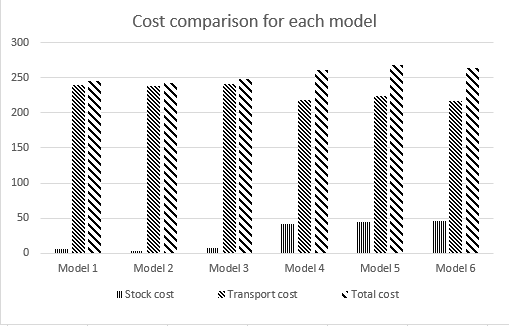
\includegraphics[width=6cm]{img/costcomparisionMODEL.png}
    \centering
    \caption{Cost comparison for each model.}
    \label{fig:ModelCosts}
\end{figure}

These results indicate that in models where delay is prioritized over warehouses or items, transport cost improves but stock cost worsens. To contrast in those models where the number of available warehouses is prioritized and the models are combined with other parameters, a stable transport cost and a significantly lower stock cost are obtained. In order to check these results, a series of metrics is obtained that allows a deeper evaluation of the stock balance in the warehouses by comparing these metrics in the greedy algorithm and the proposed one. To do this, we first obtain the average negative stock of all platforms (see Fig \ref{fig:ModelAverage}).

The average number of items with negative stock reinforces our hypothesis that the number of warehouses available per trip is a determining factor. In order to decide which model to use for the LCR list, we obtain the number of items where the stock is negative (see Fig \ref{fig:ModelItems}))

\begin{figure}[H]
    \begin{subfigure}{.5\textwidth}
        \centering
        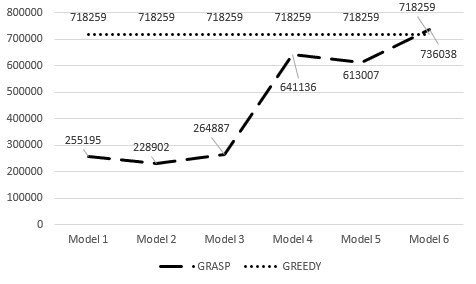
\includegraphics[ width=\linewidth]{img/averagestocknegativeMODEL.png}
        \caption{Average}
    \label{fig:ModelAverage}
    \end{subfigure}
    \begin{subfigure}{.5\textwidth}
      \centering
      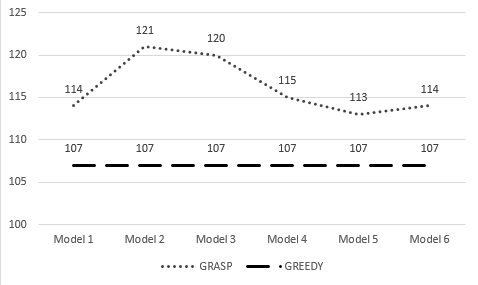
\includegraphics[ width=\linewidth]{img/itemsstocknegativeMODEL.png}
      \caption{Quantity}
    \label{fig:ModelItems}
    \end{subfigure}
    \caption{Metrics of items with negative stock for each model.}
\end{figure}
Finally, we decided to use the ordering model based on quantity of available warehouses and amount of items in the order. We selected this model because it is the one that generates the least number of items with negative stock and the lowest average of negative stock, and it keeps the cost of transport constant.

The set of improvements optimize the scheduling of the algorithm and maintain balanced stock. These improvements are evaluated by measuring metrics that are similar to those used previously. Each one of these improvements implements the previous one, because they depend on each other. In all of the improvements applied to the algorithm, they are implemented with a LCR ordering model 2. Basically, we obtain the different transport and stock costs and compare them in order to have a general view of the  impact of the improvement on the solution of the algorithm (see Fig \ref{fig:ImprovementsCosts}).

\begin{figure}[H]
    \centering
    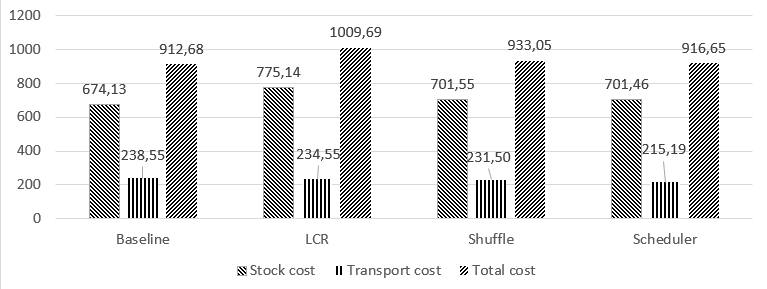
\includegraphics[width=6cm]{img/comparisoncostIMPROV.png}
    \caption{Different costs for each improvements.}
    \label{fig:ImprovementsCosts}
\end{figure}

As shown, the test results do not show significant differences in costs; only the implementation of all of the improvements slightly reduces the total cost. To ensure that the improvements used optimize the solution, we obtain metrics based on stock balancing (see Fig \ref{fig:StockBalancing}).

\begin{figure}[H]
    \begin{subfigure}{.5\textwidth}
        \centering
        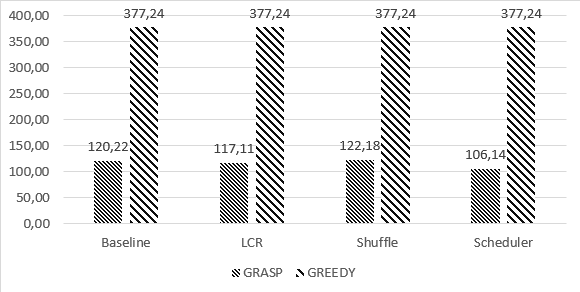
\includegraphics[ width=6cm]{img/averagestocknegativeIMPROV.png}
        \caption{Average number of items with negative stock for each improvement.}
    \end{subfigure}
    \begin{subfigure}{.5\textwidth}
      \centering
      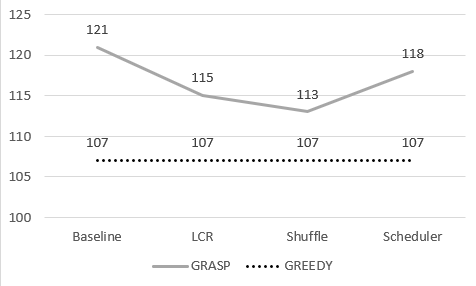
\includegraphics[ width=6cm]{img/quatitytocknegativeIMPROV.png}
      \caption{Amount of items with negative stock for each improvement}
    \end{subfigure}
    \caption{Metrics based on stock balancing}
    \label{fig:StockBalancing}
\end{figure}

The results obtained from the metrics for the evaluation of the balance of the stock show us that the average stock of the items in the warehouses remains stable with a difference of between 67\% and 71\%, while the number of items with negative stock increases with respect to the algorithm already implemented. This is a good result. If we compare the average and the amount negative stock of items at warehouses, we determine that there are more items with negative stock but the value of these is much lower. Therefore, the negative stock is balanced with the new improvements.
Finally, the two algorithms are compared completely, using the cost and stock balancing metrics used previously. First, the total cost is evaluated for the first two weeks of July 2020 (see Fig \ref{fig:weekcosts}).
The results indicate that the algorithm improves the results of the first week but worsens the second week. This is because GRASP was developed to improve the balance at the expense of the transport cost. Second, the stock metrics are evaluated to determine whether or not the algorithm balances the stocks correctly.

\begin{figure}[H]
    \begin{subfigure}{.5\textwidth}
        \centering
        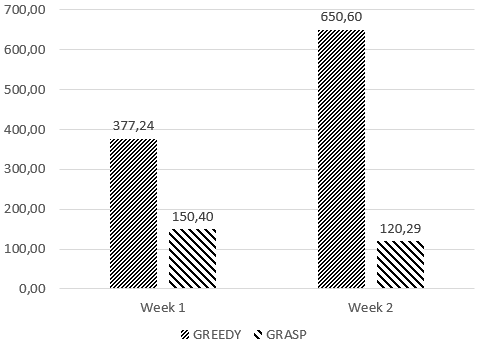
\includegraphics[width=6cm]{img/averagestocknegativeALGOTH.png}
        \caption{Average number of negative stock items.}
        \label{fig:weeksaverage}
    \end{subfigure}
    \begin{subfigure}{.5\textwidth}
      \centering
      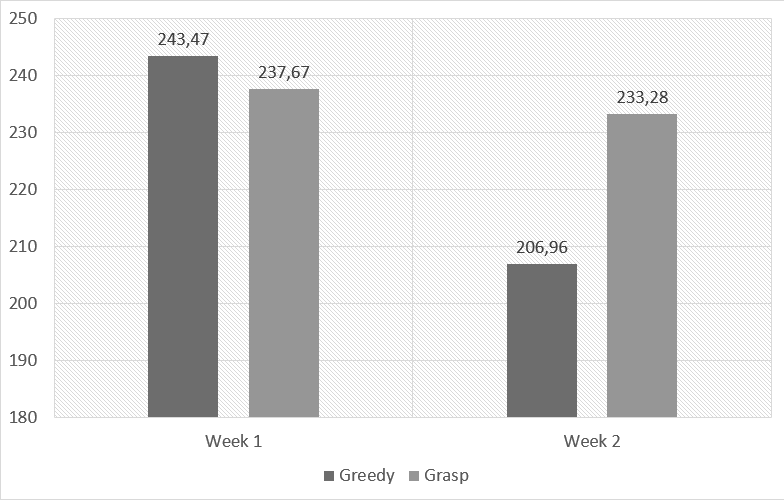
\includegraphics[width=6cm]{img/cost.png}
        \caption{Total cost comparison.}
        \label{fig:weekcosts}
    \end{subfigure}
    \caption{Metrics in the first half of July 2020.}
\end{figure}

First, a metric is shown that calculates the average negative stock amount for all of the warehouses (see Graph \ref{fig:weeksaverage}). This metric is very important because it allows us to see how the stock is distributed in the warehouses. The improvement provided by the GRASP in the average negative stock quantity is between 60\% and 81\%.
On the other hand the number of items with negative stock (see Graph \ref{fig:weeksQuantity}) is also a metric that helps us to measure the dispersion of stock among the warehouses. In this case, you can see an improvement by the GRASP of between 41\% and 60\% based on data from the greedy algorithm.
Finally, the costs of the two weeks are obtained to evaluate them jointly (see Graph \ref{fig:final})

\begin{figure}[H]
    \begin{subfigure}{.5\textwidth}
        \centering
        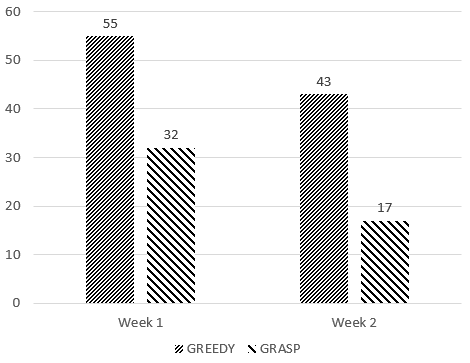
\includegraphics[width=6cm]{img/itemsstocknegativeALGOTH.png}
        \caption{Quantity of negative stock items in the first half of July 2020}
        \label{fig:weeksQuantity}
    \end{subfigure}
    \begin{subfigure}{.5\textwidth}
        \centering
        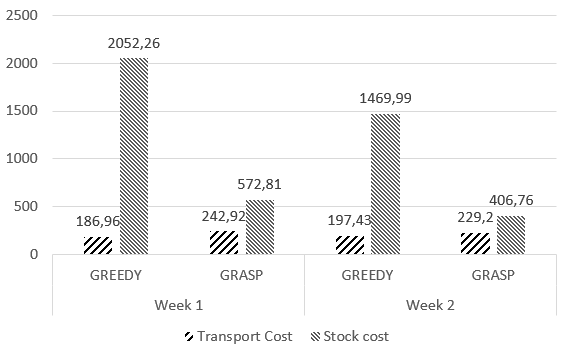
\includegraphics[ width=6cm]{img/FINAL.png}
        \caption{Stock and transport cost comparison between the greedy algorithm and GRASP}
        \label{fig:final}
    \end{subfigure}
    \caption{Metrics in the first half of July 2020.}
\end{figure}

The results show a large difference in the stock cost between the different algorithms for the two weeks shown. It can also be observed that even through the transport cost is higher in GRASP. The penalty is relatively low compared to the improvement in the stock cost. The stock cost improves by about 72\% and the transport cost worsens by between 13\% and 21\%. The computational time taken by the greedy algorithm is about 20 to 30 minutes, while GRASP takes between 0.45 and 1.5 minutes.

\section*{Conclusions and future work}


Transport companies need to optimize their logistics infrastructures and strategies in order to be more efficient in a more competitive world. This work tries to merge two different problems, the warehouse stock management problem and the routing problem in order to minimize both the negative stock and the transport cost. To do this, a GRASP-based metaheuristic has been developed to improve the greedy algorithm that is currently being used by the company. The results in several case studies show that the greedy algorithm had a better behavior in the transport cost, since it is specially guided by a heuristic. However, the proposed GRASP algorithm overcomes the results obtained by the greedy algorithm in stock balancing, improving the negative average stock by up to 82\%.

In future works, we will improve the proposed algorithm by combining the proposed GRASP algorithm with a genetic algorithm (GA). Thus, the solutions obtained by the GRASP algorithm will participate as a subset of the initial population for the genetic algorithm. This could improve the quality of the solutions due to the high capability of the GA to combine previous solutions and avoid blockage in the local optimal.


\subsection*{Acknowledgements}
The paper has been partially supported by the Spanish research project TIN2016-80856-R.

\bibliography{bib}
\bibliographystyle{aaai}
\end{document}
